\subsection{DoublyLinkedList}
\label{sec:DoublyLinkedList}
En doublylistedlist er blevet valgt til projektet da det er blevet vurderet at den har de fleste fordele i forhold til andre datastrukturer. Som der er erfaring med i gruppen, en fordel ved at holde sig til en datastruktur er mere tid til at udvikle den og lave den rigtig god i forhold til at lave mange forskellige strukturere. Den er Implementeret som en template klasse.

\begin{figure}[h]
\centering 
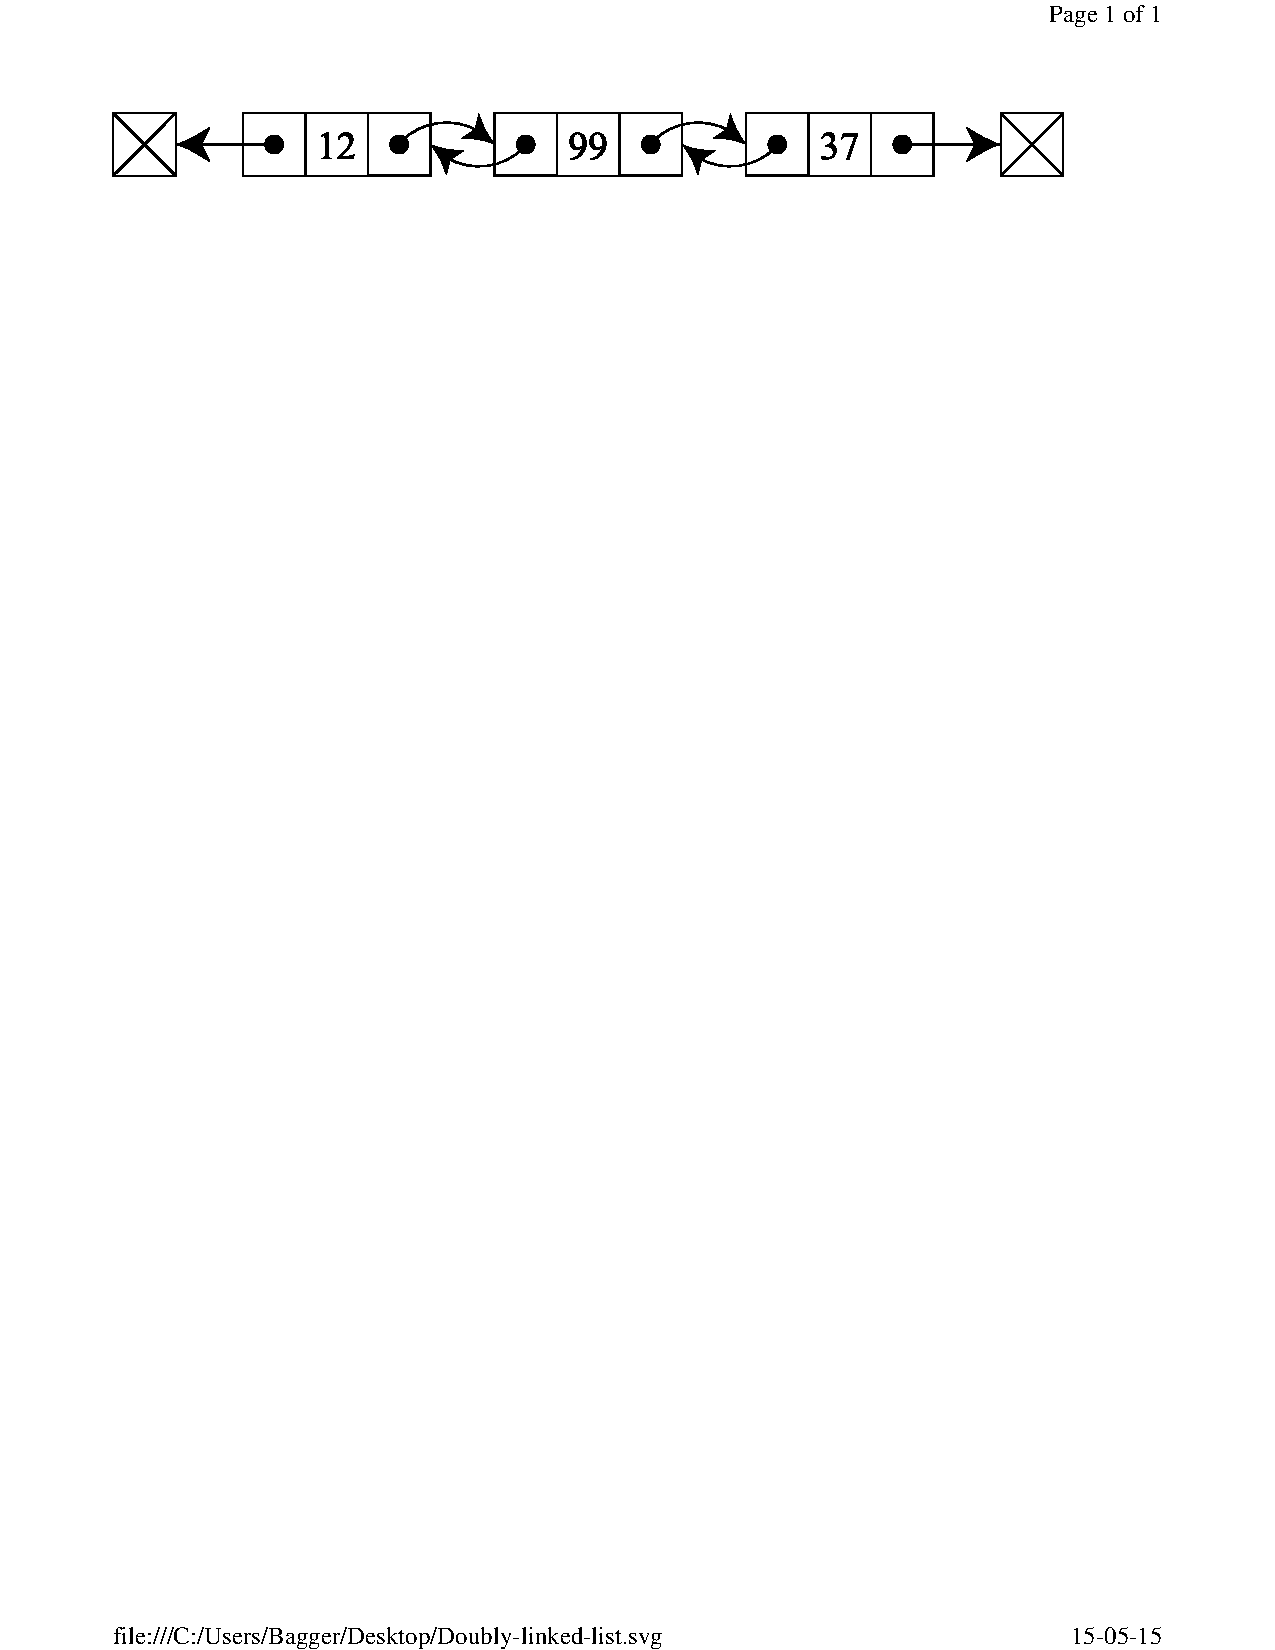
\includegraphics[width={\textwidth-2cm}, trim=0 700 0 50, clip=true] {../fig/Doubly_linked_list.pdf}
\caption{A doubly linked list whose nodes contain three fields: an integer value, the link forward to the next node, and the link backward to the previous node.}
\label{fig:doubly_linked_list}
\end{figure}

Denne kommer til at have samme struktur som Figur \ref{fig:doubly_linked_list} i stedet for kun at gemme ints laves den som en template klasse så vi kan gemme alle data typer.

\subsubsection{Attributter}

\begin{table}[h]
\begin{tabularx}{\textwidth}{| Z | Z | L{10 cm} |} \hline
\texttt{headPtr} & \texttt{Node<A\_Type>*} & Head ponteren som bruges internt i klassen, og peger på det første element i listen. \\\hline
\texttt{tailPtr} & \texttt{Node<A\_Type>*} & Tail ponteren som bruges internt i klassen, og peger på det bagerste element i listen. \\\hline
\texttt{itemsInList} & \texttt{int} & En int som holder styr på hvor mange elemeter som den doubly listed list indeholder. \\\hline
\end{tabularx}
\caption{Attributter for klassen DoublyLinkedList}
\label{table:DoublyLinkedList_attributter}
\end{table}

\subsubsection{Metoder}

\begin{table}[h]
\begin{tabularx}{\textwidth}{| L{2.5 cm} | Z |} \hline
Prototype & \texttt{DoublyLinkedList()} \\\hline
Parametre & \texttt{-}\\\hline
Returværdi & \texttt{-}\\\hline
Beskrivelse & headPtr og tailPtr sættes til at peger på NULL og itemsInList sættes til 0. \\\hline
\end{tabularx}
\caption{DoublyLinkedList}
\label{table:DoublyLinkedList_contructor}
\end{table}


\begin{table}[h]
\begin{tabularx}{\textwidth}{| L{2.5 cm} | Z |} \hline
Prototype & \texttt{\textasciitilde DoublyLinkedList()} \\\hline
Parametre & \texttt{-}\\\hline
Returværdi & \texttt{-}\\\hline
Beskrivelse & Når klassen nedlægges fjernes alt det data som den havde gemt. \\\hline
\end{tabularx}
\caption{\textasciitilde DoublyLinkedList}
\label{table:DoublyLinkedList_destructor}
\end{table}


\begin{table}[ht]
\begin{tabularx}{\textwidth}{| L{2.5 cm} | Z |} \hline
Prototype & \texttt{void tailInsert(A\_Type info)} \\\hline
Parametre & \texttt{A\_Type info} \newline
Datatypen som skal gemmes i listen. \\\hline
Returværdi & \texttt{-} \\\hline
Beskrivelse & Bruges til at gemme datatypen bagerest i listen. \\\hline
\end{tabularx}
\caption{tailInsert}
\label{table:DoublyLinkedList_tailInsert}
\end{table}

\begin{table}[ht]
\begin{tabularx}{\textwidth}{| L{2.5 cm} | Z |} \hline
Prototype & \texttt{void headInsert(A\_Type info)} \\\hline
Parametre & \texttt{A\_Type info} \newline
Datatypen som skal gemmes i listen. \\\hline
Returværdi & \texttt{-} \\\hline
Beskrivelse & Bruges til at gemme datatypen fronten i listen. \\\hline
\end{tabularx}
\caption{tailInsert}
\label{table:DoublyLinkedList_headInsert}
\end{table}

\begin{table}[ht]
\begin{tabularx}{\textwidth}{| L{2.5 cm} | Z |} \hline
Prototype & \texttt{void headDelete()} \\\hline
Parametre & \texttt{-} \\\hline
Returværdi & \texttt{-} \\\hline
Beskrivelse & Bruges til at fjerne element i fronten listen. \\\hline
\end{tabularx}
\caption{headDelete}
\label{table:DoublyLinkedList_headDelete}
\end{table}


\begin{table}[ht]
\begin{tabularx}{\textwidth}{| L{2.5 cm} | Z |} \hline
Prototype & \texttt{void tailDelete()} \\\hline
Parametre & \texttt{-} \\\hline
Returværdi & \texttt{-} \\\hline
Beskrivelse & Bruges til at fjerne det bagerste element i listen. \\\hline
\end{tabularx}
\caption{tailDelete}
\label{table:DoublyLinkedList_tailDelete}
\end{table}


\begin{table}[ht]
\begin{tabularx}{\textwidth}{| L{2.5 cm} | Z |} \hline
Prototype & \texttt{void forwardTraversing()} \\\hline
Parametre & \texttt{-} \\\hline
Returværdi & \texttt{-} \\\hline
Beskrivelse & Løber gennem hele den doubly linked list fra headPtr til tailPtr og udskriver alle elementer som den har glemt. \\\hline
\end{tabularx}
\caption{forwardTraversing}
\label{table:DoublyLinkedList_forwardTraversing}
\end{table}


\begin{table}[ht]
\begin{tabularx}{\textwidth}{| L{2.5 cm} | Z |} \hline
Prototype & \texttt{void backwardTraversing()} \\\hline
Parametre & \texttt{-} \\\hline
Returværdi & \texttt{-} \\\hline
Beskrivelse & Løber gennem hele den doubly linked list fra tailPtr til headPtr og udskriver alle elementer som den har glemt. \\\hline
\end{tabularx}
\caption{backwardTraversing}
\label{table:DoublyLinkedList_backwardTraversing}
\end{table}


\begin{table}[ht]
\begin{tabularx}{\textwidth}{| L{2.5 cm} | Z |} \hline
Prototype & \texttt{int Find(A\_Type valueToFind)} \\\hline
Parametre & \texttt{A\_Type valueToFind} \newline
En type af A\_Type som den skal prøve at finde i listen. \\\hline
Returværdi & Hvis den findes i listen returnere den et tal over 0 som angiver dens placering i listen. Hvis -1 findes den ikke i listen. \\\hline
Beskrivelse & Bruges til at finde en type af A\_Type i den linked list. \\\hline
\end{tabularx}
\caption{Find}
\label{table:DoublyLinkedList_Find}
\end{table}

\begin{table}[ht]
\begin{tabularx}{\textwidth}{| L{2.5 cm} | Z |} \hline
Prototype & \texttt{int PeekTail(A\_Type \&PeekTail)} \\\hline
Parametre & \texttt{A\_Type \&PeekTail} \newline
En reference til en A\_Type, som ændres til det element som tailPtr peger på. \\\hline
Returværdi & Hvis der er noget indhold i listen får man 1 tilbage ellers -1. \\\hline
Beskrivelse & Anvendes til at hente det element som ligger bagerst i listen. \\\hline
\end{tabularx}
\caption{PeekTail}
\label{table:DoublyLinkedList_PeekTail}
\end{table}


\begin{table}[ht]
\begin{tabularx}{\textwidth}{| L{2.5 cm} | Z |} \hline
Prototype & \texttt{int PeekHead(A\_Type \&PeekHead)} \\\hline
Parametre & \texttt{A\_Type \&PeekHead} \newline
En reference til en A\_Type, som ændres til det element som headPtr peger på. \\\hline
Returværdi & Hvis der er noget indhold i listen får man 1 tilbage ellers -1. \\\hline
Beskrivelse & Anvendes til at hente det element som ligger fronten i listen. \\\hline
\end{tabularx}
\caption{PeekHead}
\label{table:DoublyLinkedList_PeekHead}
\end{table}


\begin{table}[ht]
\begin{tabularx}{\textwidth}{| L{2.5 cm} | Z |} \hline
Prototype & \texttt{void deleteAt(int place)} \\\hline
Parametre & \texttt{int place} \newline
En placering i listen, som angiver det sted, hvor et element som ønskes slettet. \\\hline
Returværdi & \texttt{-} \\\hline
Beskrivelse & Bruges et at slette et element på den plads som parlamenteren angiver. \\\hline
\end{tabularx}
\caption{deleteAt}
\label{table:DoublyLinkedList_deleteAt}
\end{table}


\begin{table}[ht]
\begin{tabularx}{\textwidth}{| L{2.5 cm} | Z |} \hline
Prototype & \texttt{int GetItemsInList()} \\\hline
Parametre & \texttt{-} \\\hline
Returværdi & Et tal som beskriver hvor mange elementer som er gemt i listen. \\\hline
Beskrivelse & Bruges til at se hvor mange elementer der er gemt i listen. \\\hline
\end{tabularx}
\caption{GetItemsInList}
\label{table:DoublyLinkedList_GetItemsInList}
\end{table}
